\documentclass[12pt]{article}
\usepackage{tikz}
\usepackage{amsmath}
% Underlining package
\usepackage{ulem}
\usetikzlibrary{calc}
\usetikzlibrary{angles,quotes}
\usepackage[a4paper, portrait, margin=1cm]{geometry}
\usepackage{fancyhdr}

\newcommand{\HeadingQuestions}{%
\section*{\Large Name: \underline{\hspace{8cm}} \hfill Date: \underline{\hspace{3cm}}}%
\vspace{-3mm}\par
\textbf{Area of a Circle}\vspace{1pt}\hrule
}

% raise footer with page number; no header
\fancypagestyle{myfancypagestyle}{
  \fancyhf{}% clear all header and footer fields
  \renewcommand{\headrulewidth}{0pt} % no rule under header
  \fancyfoot[C] {\thepage} \setlength{\footskip}{14.5pt} % raise page number allowed min 14.5pt
}
\pagestyle{myfancypagestyle}  % apply myfancypagestyle

\newcounter{minipagecount}

\begin{document}
\HeadingQuestions
\vspace{8mm}

\begin{minipage}{0.55\textwidth}
  \refstepcounter{minipagecount}
  \noindent{(\theminipagecount)}\quad
  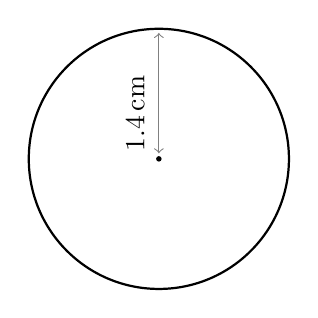
\begin{tikzpicture}[scale=1.0, baseline=(current bounding box.north)]
    \begin{scope}[rotate=0]
        \coordinate (A) at (0,0);
        % Define B using polar coordinates from A
        \coordinate (B) at ($(A) + (90:1.652)$);
        \fill (A) circle(1pt);
        \draw[thick] (A) circle (1.652);
        \draw[<->, gray, shorten <=2pt, shorten >=1.5pt]
          (A) -- (B)
          node[pos=0.35, sloped, above, fill=white, inner sep=2pt, xshift=0pt, yshift=3pt, transform shape]
          {\textcolor{black}{$1.4\,\text{cm}$}};
    \end{scope}
  \end{tikzpicture}
\end{minipage}%
\hfill
\begin{minipage}{.4\textwidth}
  \begin{align*}
  \text{Area} &= \pi r^2 \\
  \text{Area} &= \pi \times (\dotuline{~~~~~~~~~~~~}\,\text{cm})^2 \\
  \text{Area} &\approx \dotuline{~~~~~~~~~~~~} \,\text{cm}^2
  \end{align*}
\end{minipage}
\par\vspace{1cm}\begin{minipage}{0.55\textwidth}
  \refstepcounter{minipagecount}
  \noindent{(\theminipagecount)}\quad
  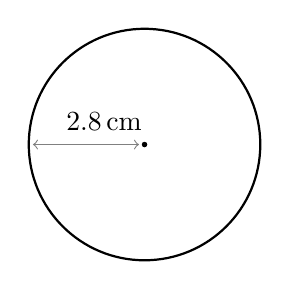
\begin{tikzpicture}[scale=1.0, baseline=(current bounding box.north)]
    \begin{scope}[rotate=0]
        \coordinate (A) at (0,0);
        % Define B using polar coordinates from A
        \coordinate (B) at ($(A) + (180:1.47)$);
        \fill (A) circle(1pt);
        \draw[thick] (A) circle (1.47);
        \draw[<->, gray, shorten <=2pt, shorten >=1.5pt]
          (A) -- (B)
          node[pos=0.35, sloped, above, fill=white, inner sep=2pt, xshift=0pt, yshift=3pt, transform shape]
          {\textcolor{black}{$2.8\,\text{cm}$}};
    \end{scope}
  \end{tikzpicture}
\end{minipage}%
\hfill
\begin{minipage}{.4\textwidth}
  \begin{align*}
  \text{Area} &= \pi r^2 \\
  \text{Area} &= \pi \times (\dotuline{~~~~~~~~~~~~}\,\text{cm})^2 \\
  \text{Area} &\approx \dotuline{~~~~~~~~~~~~} \,\text{cm}^2
  \end{align*}
\end{minipage}
\par\vspace{1cm}\begin{minipage}{0.55\textwidth}
  \refstepcounter{minipagecount}
  \noindent{(\theminipagecount)}\quad
  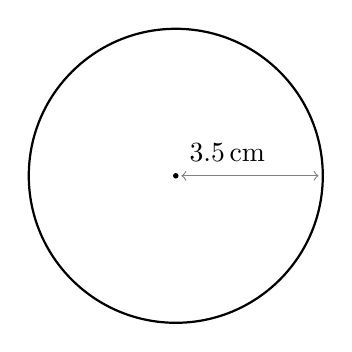
\begin{tikzpicture}[scale=1.0, baseline=(current bounding box.north)]
    \begin{scope}[rotate=0]
        \coordinate (A) at (0,0);
        % Define B using polar coordinates from A
        \coordinate (B) at ($(A) + (0:1.867)$);
        \fill (A) circle(1pt);
        \draw[thick] (A) circle (1.867);
        \draw[<->, gray, shorten <=2pt, shorten >=1.5pt]
          (A) -- (B)
          node[pos=0.35, sloped, above, fill=white, inner sep=2pt, xshift=0pt, yshift=3pt, transform shape]
          {\textcolor{black}{$3.5\,\text{cm}$}};
    \end{scope}
  \end{tikzpicture}
\end{minipage}%
\hfill
\begin{minipage}{.4\textwidth}
  \begin{align*}
  \text{Area} &= \pi r^2 \\
  \text{Area} &= \pi \times (\dotuline{~~~~~~~~~~~~}\,\text{cm})^2 \\
  \text{Area} &\approx \dotuline{~~~~~~~~~~~~} \,\text{cm}^2
  \end{align*}
\end{minipage}
\par\vspace{1cm}\begin{minipage}{0.55\textwidth}
  \refstepcounter{minipagecount}
  \noindent{(\theminipagecount)}\quad
  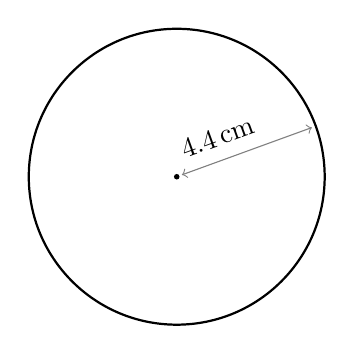
\begin{tikzpicture}[scale=1.0, baseline=(current bounding box.north)]
    \begin{scope}[rotate=0]
        \coordinate (A) at (0,0);
        % Define B using polar coordinates from A
        \coordinate (B) at ($(A) + (20:1.879)$);
        \fill (A) circle(1pt);
        \draw[thick] (A) circle (1.879);
        \draw[<->, gray, shorten <=2pt, shorten >=1.5pt]
          (A) -- (B)
          node[pos=0.35, sloped, above, fill=white, inner sep=2pt, xshift=0pt, yshift=3pt, transform shape]
          {\textcolor{black}{$4.4\,\text{cm}$}};
    \end{scope}
  \end{tikzpicture}
\end{minipage}%
\hfill
\begin{minipage}{.4\textwidth}
  \begin{align*}
  \text{Area} &= \pi r^2 \\
  \text{Area} &= \pi \times (\dotuline{~~~~~~~~~~~~}\,\text{cm})^2 \\
  \text{Area} &\approx \dotuline{~~~~~~~~~~~~} \,\text{cm}^2
  \end{align*}
\end{minipage}
\par\vspace{1cm}\begin{minipage}{0.55\textwidth}
  \refstepcounter{minipagecount}
  \noindent{(\theminipagecount)}\quad
  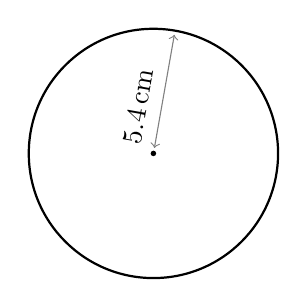
\begin{tikzpicture}[scale=1.0, baseline=(current bounding box.north)]
    \begin{scope}[rotate=0]
        \coordinate (A) at (0,0);
        % Define B using polar coordinates from A
        \coordinate (B) at ($(A) + (80:1.583)$);
        \fill (A) circle(1pt);
        \draw[thick] (A) circle (1.583);
        \draw[<->, gray, shorten <=2pt, shorten >=1.5pt]
          (A) -- (B)
          node[pos=0.35, sloped, above, fill=white, inner sep=2pt, xshift=0pt, yshift=3pt, transform shape]
          {\textcolor{black}{$5.4\,\text{cm}$}};
    \end{scope}
  \end{tikzpicture}
\end{minipage}%
\hfill
\begin{minipage}{.4\textwidth}
  \begin{align*}
  \text{Area} &= \pi r^2 \\
  \text{Area} &= \pi \times (\dotuline{~~~~~~~~~~~~}\,\text{cm})^2 \\
  \text{Area} &\approx \dotuline{~~~~~~~~~~~~} \,\text{cm}^2
  \end{align*}
\end{minipage}
\par\vspace{1cm}\begin{minipage}{0.55\textwidth}
  \refstepcounter{minipagecount}
  \noindent{(\theminipagecount)}\quad
  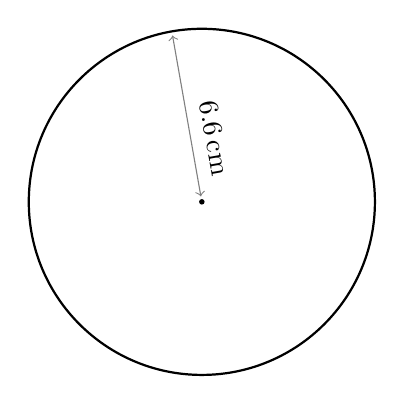
\begin{tikzpicture}[scale=1.0, baseline=(current bounding box.north)]
    \begin{scope}[rotate=0]
        \coordinate (A) at (0,0);
        % Define B using polar coordinates from A
        \coordinate (B) at ($(A) + (100:2.198)$);
        \fill (A) circle(1pt);
        \draw[thick] (A) circle (2.198);
        \draw[<->, gray, shorten <=2pt, shorten >=1.5pt]
          (A) -- (B)
          node[pos=0.35, sloped, above, fill=white, inner sep=2pt, xshift=0pt, yshift=3pt, transform shape]
          {\textcolor{black}{$6.6\,\text{cm}$}};
    \end{scope}
  \end{tikzpicture}
\end{minipage}%
\hfill
\begin{minipage}{.4\textwidth}
  \begin{align*}
  \text{Area} &= \pi r^2 \\
  \text{Area} &= \pi \times (\dotuline{~~~~~~~~~~~~}\,\text{cm})^2 \\
  \text{Area} &\approx \dotuline{~~~~~~~~~~~~} \,\text{cm}^2
  \end{align*}
\end{minipage}
\par\vspace{1cm}\begin{minipage}{0.55\textwidth}
  \refstepcounter{minipagecount}
  \noindent{(\theminipagecount)}\quad
  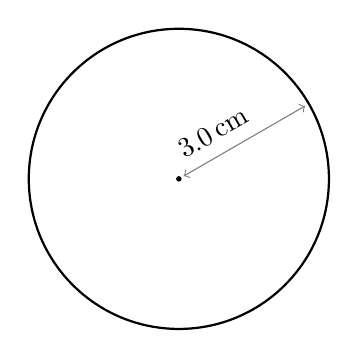
\begin{tikzpicture}[scale=1.0, baseline=(current bounding box.north)]
    \begin{scope}[rotate=0]
        \coordinate (A) at (0,0);
        % Define B using polar coordinates from A
        \coordinate (B) at ($(A) + (30:1.906)$);
        \fill (A) circle(1pt);
        \draw[thick] (A) circle (1.906);
        \draw[<->, gray, shorten <=2pt, shorten >=1.5pt]
          (A) -- (B)
          node[pos=0.35, sloped, above, fill=white, inner sep=2pt, xshift=0pt, yshift=3pt, transform shape]
          {\textcolor{black}{$3.0\,\text{cm}$}};
    \end{scope}
  \end{tikzpicture}
\end{minipage}%
\hfill
\begin{minipage}{.4\textwidth}
  \begin{align*}
  \text{Area} &= \pi r^2 \\
  \text{Area} &= \pi \times (\dotuline{~~~~~~~~~~~~}\,\text{cm})^2 \\
  \text{Area} &\approx \dotuline{~~~~~~~~~~~~} \,\text{cm}^2
  \end{align*}
\end{minipage}
\par\vspace{1cm}\begin{minipage}{0.55\textwidth}
  \refstepcounter{minipagecount}
  \noindent{(\theminipagecount)}\quad
  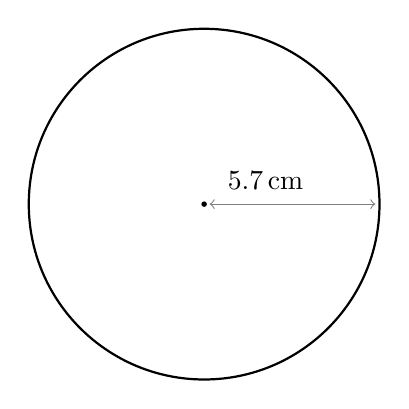
\begin{tikzpicture}[scale=1.0, baseline=(current bounding box.north)]
    \begin{scope}[rotate=0]
        \coordinate (A) at (0,0);
        % Define B using polar coordinates from A
        \coordinate (B) at ($(A) + (0:2.227)$);
        \fill (A) circle(1pt);
        \draw[thick] (A) circle (2.227);
        \draw[<->, gray, shorten <=2pt, shorten >=1.5pt]
          (A) -- (B)
          node[pos=0.35, sloped, above, fill=white, inner sep=2pt, xshift=0pt, yshift=3pt, transform shape]
          {\textcolor{black}{$5.7\,\text{cm}$}};
    \end{scope}
  \end{tikzpicture}
\end{minipage}%
\hfill
\begin{minipage}{.4\textwidth}
  \begin{align*}
  \text{Area} &= \pi r^2 \\
  \text{Area} &= \pi \times (\dotuline{~~~~~~~~~~~~}\,\text{cm})^2 \\
  \text{Area} &\approx \dotuline{~~~~~~~~~~~~} \,\text{cm}^2
  \end{align*}
\end{minipage}
\par\vspace{1cm}\begin{minipage}{0.55\textwidth}
  \refstepcounter{minipagecount}
  \noindent{(\theminipagecount)}\quad
  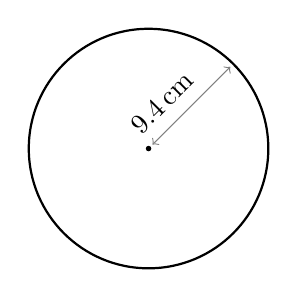
\begin{tikzpicture}[scale=1.0, baseline=(current bounding box.north)]
    \begin{scope}[rotate=0]
        \coordinate (A) at (0,0);
        % Define B using polar coordinates from A
        \coordinate (B) at ($(A) + (45:1.521)$);
        \fill (A) circle(1pt);
        \draw[thick] (A) circle (1.521);
        \draw[<->, gray, shorten <=2pt, shorten >=1.5pt]
          (A) -- (B)
          node[pos=0.35, sloped, above, fill=white, inner sep=2pt, xshift=0pt, yshift=3pt, transform shape]
          {\textcolor{black}{$9.4\,\text{cm}$}};
    \end{scope}
  \end{tikzpicture}
\end{minipage}%
\hfill
\begin{minipage}{.4\textwidth}
  \begin{align*}
  \text{Area} &= \pi r^2 \\
  \text{Area} &= \pi \times (\dotuline{~~~~~~~~~~~~}\,\text{cm})^2 \\
  \text{Area} &\approx \dotuline{~~~~~~~~~~~~} \,\text{cm}^2
  \end{align*}
\end{minipage}
\par\vspace{1cm}\begin{minipage}{0.55\textwidth}
  \refstepcounter{minipagecount}
  \noindent{(\theminipagecount)}\quad
  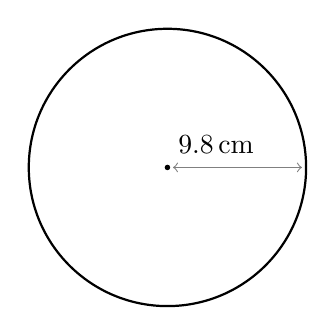
\begin{tikzpicture}[scale=1.0, baseline=(current bounding box.north)]
    \begin{scope}[rotate=0]
        \coordinate (A) at (0,0);
        % Define B using polar coordinates from A
        \coordinate (B) at ($(A) + (0:1.761)$);
        \fill (A) circle(1pt);
        \draw[thick] (A) circle (1.761);
        \draw[<->, gray, shorten <=2pt, shorten >=1.5pt]
          (A) -- (B)
          node[pos=0.35, sloped, above, fill=white, inner sep=2pt, xshift=0pt, yshift=3pt, transform shape]
          {\textcolor{black}{$9.8\,\text{cm}$}};
    \end{scope}
  \end{tikzpicture}
\end{minipage}%
\hfill
\begin{minipage}{.4\textwidth}
  \begin{align*}
  \text{Area} &= \pi r^2 \\
  \text{Area} &= \pi \times (\dotuline{~~~~~~~~~~~~}\,\text{cm})^2 \\
  \text{Area} &\approx \dotuline{~~~~~~~~~~~~} \,\text{cm}^2
  \end{align*}
\end{minipage}
\par\vspace{1cm}\begin{minipage}{0.55\textwidth}
  \refstepcounter{minipagecount}
  \noindent{(\theminipagecount)}\quad
  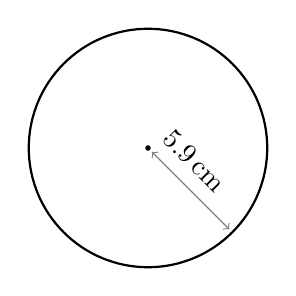
\begin{tikzpicture}[scale=1.0, baseline=(current bounding box.north)]
    \begin{scope}[rotate=0]
        \coordinate (A) at (0,0);
        % Define B using polar coordinates from A
        \coordinate (B) at ($(A) + (315:1.514)$);
        \fill (A) circle(1pt);
        \draw[thick] (A) circle (1.514);
        \draw[<->, gray, shorten <=2pt, shorten >=1.5pt]
          (A) -- (B)
          node[pos=0.35, sloped, above, fill=white, inner sep=2pt, xshift=0pt, yshift=3pt, transform shape]
          {\textcolor{black}{$5.9\,\text{cm}$}};
    \end{scope}
  \end{tikzpicture}
\end{minipage}%
\hfill
\begin{minipage}{.4\textwidth}
  \begin{align*}
  \text{Area} &= \pi r^2 \\
  \text{Area} &= \pi \times (\dotuline{~~~~~~~~~~~~}\,\text{cm})^2 \\
  \text{Area} &\approx \dotuline{~~~~~~~~~~~~} \,\text{cm}^2
  \end{align*}
\end{minipage}
\par\vspace{1cm}\begin{minipage}{0.55\textwidth}
  \refstepcounter{minipagecount}
  \noindent{(\theminipagecount)}\quad
  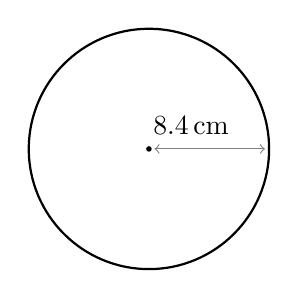
\begin{tikzpicture}[scale=1.0, baseline=(current bounding box.north)]
    \begin{scope}[rotate=0]
        \coordinate (A) at (0,0);
        % Define B using polar coordinates from A
        \coordinate (B) at ($(A) + (0:1.526)$);
        \fill (A) circle(1pt);
        \draw[thick] (A) circle (1.526);
        \draw[<->, gray, shorten <=2pt, shorten >=1.5pt]
          (A) -- (B)
          node[pos=0.35, sloped, above, fill=white, inner sep=2pt, xshift=0pt, yshift=3pt, transform shape]
          {\textcolor{black}{$8.4\,\text{cm}$}};
    \end{scope}
  \end{tikzpicture}
\end{minipage}%
\hfill
\begin{minipage}{.4\textwidth}
  \begin{align*}
  \text{Area} &= \pi r^2 \\
  \text{Area} &= \pi \times (\dotuline{~~~~~~~~~~~~}\,\text{cm})^2 \\
  \text{Area} &\approx \dotuline{~~~~~~~~~~~~} \,\text{cm}^2
  \end{align*}
\end{minipage}
\par\vspace{1cm}\begin{minipage}{0.55\textwidth}
  \refstepcounter{minipagecount}
  \noindent{(\theminipagecount)}\quad
  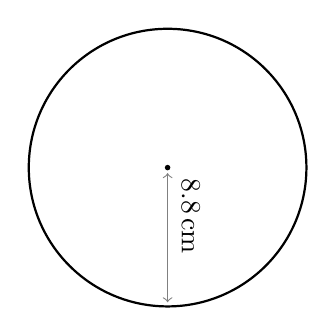
\begin{tikzpicture}[scale=1.0, baseline=(current bounding box.north)]
    \begin{scope}[rotate=0]
        \coordinate (A) at (0,0);
        % Define B using polar coordinates from A
        \coordinate (B) at ($(A) + (270:1.763)$);
        \fill (A) circle(1pt);
        \draw[thick] (A) circle (1.763);
        \draw[<->, gray, shorten <=2pt, shorten >=1.5pt]
          (A) -- (B)
          node[pos=0.35, sloped, above, fill=white, inner sep=2pt, xshift=0pt, yshift=3pt, transform shape]
          {\textcolor{black}{$8.8\,\text{cm}$}};
    \end{scope}
  \end{tikzpicture}
\end{minipage}%
\hfill
\begin{minipage}{.4\textwidth}
  \begin{align*}
  \text{Area} &= \pi r^2 \\
  \text{Area} &= \pi \times (\dotuline{~~~~~~~~~~~~}\,\text{cm})^2 \\
  \text{Area} &\approx \dotuline{~~~~~~~~~~~~} \,\text{cm}^2
  \end{align*}
\end{minipage}
\par\vspace{1cm}\begin{minipage}{0.55\textwidth}
  \refstepcounter{minipagecount}
  \noindent{(\theminipagecount)}\quad
  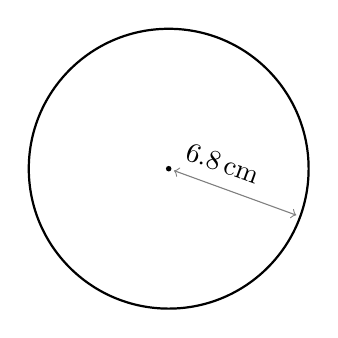
\begin{tikzpicture}[scale=1.0, baseline=(current bounding box.north)]
    \begin{scope}[rotate=0]
        \coordinate (A) at (0,0);
        % Define B using polar coordinates from A
        \coordinate (B) at ($(A) + (-20:1.777)$);
        \fill (A) circle(1pt);
        \draw[thick] (A) circle (1.777);
        \draw[<->, gray, shorten <=2pt, shorten >=1.5pt]
          (A) -- (B)
          node[pos=0.35, sloped, above, fill=white, inner sep=2pt, xshift=0pt, yshift=3pt, transform shape]
          {\textcolor{black}{$6.8\,\text{cm}$}};
    \end{scope}
  \end{tikzpicture}
\end{minipage}%
\hfill
\begin{minipage}{.4\textwidth}
  \begin{align*}
  \text{Area} &= \pi r^2 \\
  \text{Area} &= \pi \times (\dotuline{~~~~~~~~~~~~}\,\text{cm})^2 \\
  \text{Area} &\approx \dotuline{~~~~~~~~~~~~} \,\text{cm}^2
  \end{align*}
\end{minipage}
\par\vspace{1cm}\begin{minipage}{0.55\textwidth}
  \refstepcounter{minipagecount}
  \noindent{(\theminipagecount)}\quad
  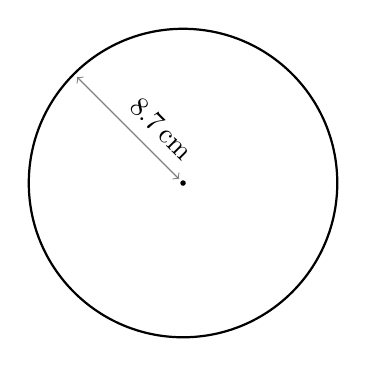
\begin{tikzpicture}[scale=1.0, baseline=(current bounding box.north)]
    \begin{scope}[rotate=0]
        \coordinate (A) at (0,0);
        % Define B using polar coordinates from A
        \coordinate (B) at ($(A) + (135:1.959)$);
        \fill (A) circle(1pt);
        \draw[thick] (A) circle (1.959);
        \draw[<->, gray, shorten <=2pt, shorten >=1.5pt]
          (A) -- (B)
          node[pos=0.35, sloped, above, fill=white, inner sep=2pt, xshift=0pt, yshift=3pt, transform shape]
          {\textcolor{black}{$8.7\,\text{cm}$}};
    \end{scope}
  \end{tikzpicture}
\end{minipage}%
\hfill
\begin{minipage}{.4\textwidth}
  \begin{align*}
  \text{Area} &= \pi r^2 \\
  \text{Area} &= \pi \times (\dotuline{~~~~~~~~~~~~}\,\text{cm})^2 \\
  \text{Area} &\approx \dotuline{~~~~~~~~~~~~} \,\text{cm}^2
  \end{align*}
\end{minipage}
\par\vspace{1cm}\begin{minipage}{0.55\textwidth}
  \refstepcounter{minipagecount}
  \noindent{(\theminipagecount)}\quad
  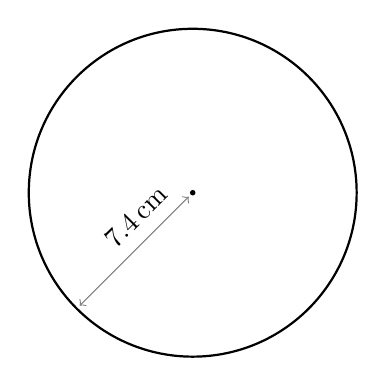
\begin{tikzpicture}[scale=1.0, baseline=(current bounding box.north)]
    \begin{scope}[rotate=0]
        \coordinate (A) at (0,0);
        % Define B using polar coordinates from A
        \coordinate (B) at ($(A) + (225:2.082)$);
        \fill (A) circle(1pt);
        \draw[thick] (A) circle (2.082);
        \draw[<->, gray, shorten <=2pt, shorten >=1.5pt]
          (A) -- (B)
          node[pos=0.35, sloped, above, fill=white, inner sep=2pt, xshift=0pt, yshift=3pt, transform shape]
          {\textcolor{black}{$7.4\,\text{cm}$}};
    \end{scope}
  \end{tikzpicture}
\end{minipage}%
\hfill
\begin{minipage}{.4\textwidth}
  \begin{align*}
  \text{Area} &= \pi r^2 \\
  \text{Area} &= \pi \times (\dotuline{~~~~~~~~~~~~}\,\text{cm})^2 \\
  \text{Area} &\approx \dotuline{~~~~~~~~~~~~} \,\text{cm}^2
  \end{align*}
\end{minipage}
\par\vspace{1cm}\begin{minipage}{0.55\textwidth}
  \refstepcounter{minipagecount}
  \noindent{(\theminipagecount)}\quad
  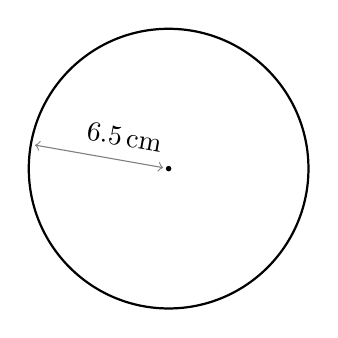
\begin{tikzpicture}[scale=1.0, baseline=(current bounding box.north)]
    \begin{scope}[rotate=0]
        \coordinate (A) at (0,0);
        % Define B using polar coordinates from A
        \coordinate (B) at ($(A) + (170:1.776)$);
        \fill (A) circle(1pt);
        \draw[thick] (A) circle (1.776);
        \draw[<->, gray, shorten <=2pt, shorten >=1.5pt]
          (A) -- (B)
          node[pos=0.35, sloped, above, fill=white, inner sep=2pt, xshift=0pt, yshift=3pt, transform shape]
          {\textcolor{black}{$6.5\,\text{cm}$}};
    \end{scope}
  \end{tikzpicture}
\end{minipage}%
\hfill
\begin{minipage}{.4\textwidth}
  \begin{align*}
  \text{Area} &= \pi r^2 \\
  \text{Area} &= \pi \times (\dotuline{~~~~~~~~~~~~}\,\text{cm})^2 \\
  \text{Area} &\approx \dotuline{~~~~~~~~~~~~} \,\text{cm}^2
  \end{align*}
\end{minipage}
\par\vspace{1cm}\begin{minipage}{0.55\textwidth}
  \refstepcounter{minipagecount}
  \noindent{(\theminipagecount)}\quad
  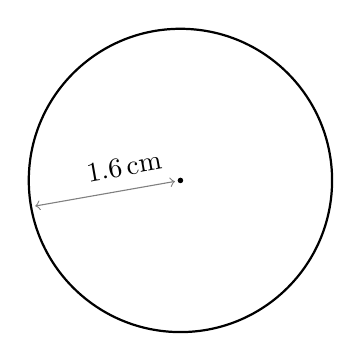
\begin{tikzpicture}[scale=1.0, baseline=(current bounding box.north)]
    \begin{scope}[rotate=0]
        \coordinate (A) at (0,0);
        % Define B using polar coordinates from A
        \coordinate (B) at ($(A) + (190:1.926)$);
        \fill (A) circle(1pt);
        \draw[thick] (A) circle (1.926);
        \draw[<->, gray, shorten <=2pt, shorten >=1.5pt]
          (A) -- (B)
          node[pos=0.35, sloped, above, fill=white, inner sep=2pt, xshift=0pt, yshift=3pt, transform shape]
          {\textcolor{black}{$1.6\,\text{cm}$}};
    \end{scope}
  \end{tikzpicture}
\end{minipage}%
\hfill
\begin{minipage}{.4\textwidth}
  \begin{align*}
  \text{Area} &= \pi r^2 \\
  \text{Area} &= \pi \times (\dotuline{~~~~~~~~~~~~}\,\text{cm})^2 \\
  \text{Area} &\approx \dotuline{~~~~~~~~~~~~} \,\text{cm}^2
  \end{align*}
\end{minipage}
\par\vspace{1cm}\begin{minipage}{0.55\textwidth}
  \refstepcounter{minipagecount}
  \noindent{(\theminipagecount)}\quad
  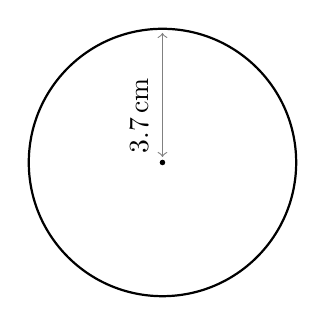
\begin{tikzpicture}[scale=1.0, baseline=(current bounding box.north)]
    \begin{scope}[rotate=0]
        \coordinate (A) at (0,0);
        % Define B using polar coordinates from A
        \coordinate (B) at ($(A) + (90:1.698)$);
        \fill (A) circle(1pt);
        \draw[thick] (A) circle (1.698);
        \draw[<->, gray, shorten <=2pt, shorten >=1.5pt]
          (A) -- (B)
          node[pos=0.35, sloped, above, fill=white, inner sep=2pt, xshift=0pt, yshift=3pt, transform shape]
          {\textcolor{black}{$3.7\,\text{cm}$}};
    \end{scope}
  \end{tikzpicture}
\end{minipage}%
\hfill
\begin{minipage}{.4\textwidth}
  \begin{align*}
  \text{Area} &= \pi r^2 \\
  \text{Area} &= \pi \times (\dotuline{~~~~~~~~~~~~}\,\text{cm})^2 \\
  \text{Area} &\approx \dotuline{~~~~~~~~~~~~} \,\text{cm}^2
  \end{align*}
\end{minipage}
\par\vspace{1cm}\begin{minipage}{0.55\textwidth}
  \refstepcounter{minipagecount}
  \noindent{(\theminipagecount)}\quad
  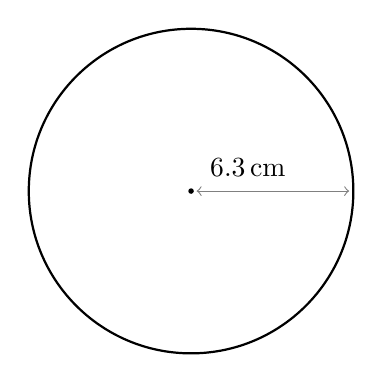
\begin{tikzpicture}[scale=1.0, baseline=(current bounding box.north)]
    \begin{scope}[rotate=0]
        \coordinate (A) at (0,0);
        % Define B using polar coordinates from A
        \coordinate (B) at ($(A) + (0:2.061)$);
        \fill (A) circle(1pt);
        \draw[thick] (A) circle (2.061);
        \draw[<->, gray, shorten <=2pt, shorten >=1.5pt]
          (A) -- (B)
          node[pos=0.35, sloped, above, fill=white, inner sep=2pt, xshift=0pt, yshift=3pt, transform shape]
          {\textcolor{black}{$6.3\,\text{cm}$}};
    \end{scope}
  \end{tikzpicture}
\end{minipage}%
\hfill
\begin{minipage}{.4\textwidth}
  \begin{align*}
  \text{Area} &= \pi r^2 \\
  \text{Area} &= \pi \times (\dotuline{~~~~~~~~~~~~}\,\text{cm})^2 \\
  \text{Area} &\approx \dotuline{~~~~~~~~~~~~} \,\text{cm}^2
  \end{align*}
\end{minipage}
\par\vspace{1cm}

\end{document}
